\section{Introduction}
\subsection{Objectifs}

Nous avons choisi de développer une \textbf{application dédiée à la reconnaissance automatique des constellations} dans le ciel nocturne. Des applications connues de reconnaissance de constellation existent déjà comme SkyView, cependant, elles utilisent uniquement la position de la constellation à une certaine période. Nous avions dès le début la volonté \textbf{d'utiliser des méthodes courantes chez les astronomes}. Ainsi, nous nous sommes orientés vers la reconnaissance automatique des constellations à partir \textbf{d’algorithmes d’analyse spatiale (pattern matching)} en utilisant l'outil préféré des astronomes : \textbf{La Géométrie}.

\subsection{Contexte}
\textbf{Astrométrie et Alignement}

\noindent Lors de l'observation astronomique, il est \textbf{crucial de savoir précisément quelles parties du ciel sont observées}. Cela permet de corréler les observations avec des catalogues d'étoiles. Contrairement à de nombreux objets de la nature \textbf{les constellations,} du fait de leur éloignement conséquent\textbf{, ne se déforment pas selon la position depuis laquelle on les observe}. Seule leur luminosité varie et  \textbf{on peut repérer avec précision la position des constellations en fonction de la période de l'année} (rotation de la Terre autour de son axe passant par l'étoile Polaire). 

\noindent Les astronomes identifient les étoiles du ciel pour déterminer la position et l'orientation d'un télescope ou d'une caméra, \textbf{créer de cartes précises du ciel} ou encore \textbf{se repérer en mer grâce au ciel}. Les astronomes amateurs contribuent grandement à la recherche en Cosmologie. Leur aide pour l’observation de phénomènes répétitifs ou pour des surveillances systématiques en prévision de comètes ou de supernovae est essentielle tant les chercheurs manquent de temps pour les réaliser.

\subsection{Plan \& Recettes}  

\noindent Voici les étapes que nous avons suivi ainsi que leur recette :

\textbf{Extraction d'étoiles} 

\noindent \textbf{Extraire} les points lumineux d'une image, 

\noindent \textbf{Retourner} les coordonnées précises et les caractéristiques des étoiles  avec une liste d'adjacence.

\textbf{Correspondance avec la base de données}

\noindent \textbf{Créer} des triangles à partir de points, 

\noindent \textbf{Retourner} le nom de la constellation la plus similaire présente dans la base de données.

\textbf{Interface}

\noindent \textbf{Afficher} l'image correspondante à la photographie dans la base de données ainsi qu'un texte original décrivant succinctement la constellation.

\subsubsection{Reconnaissance Automatique de Constellations}

\begin{figure}[ht]
    \centering
    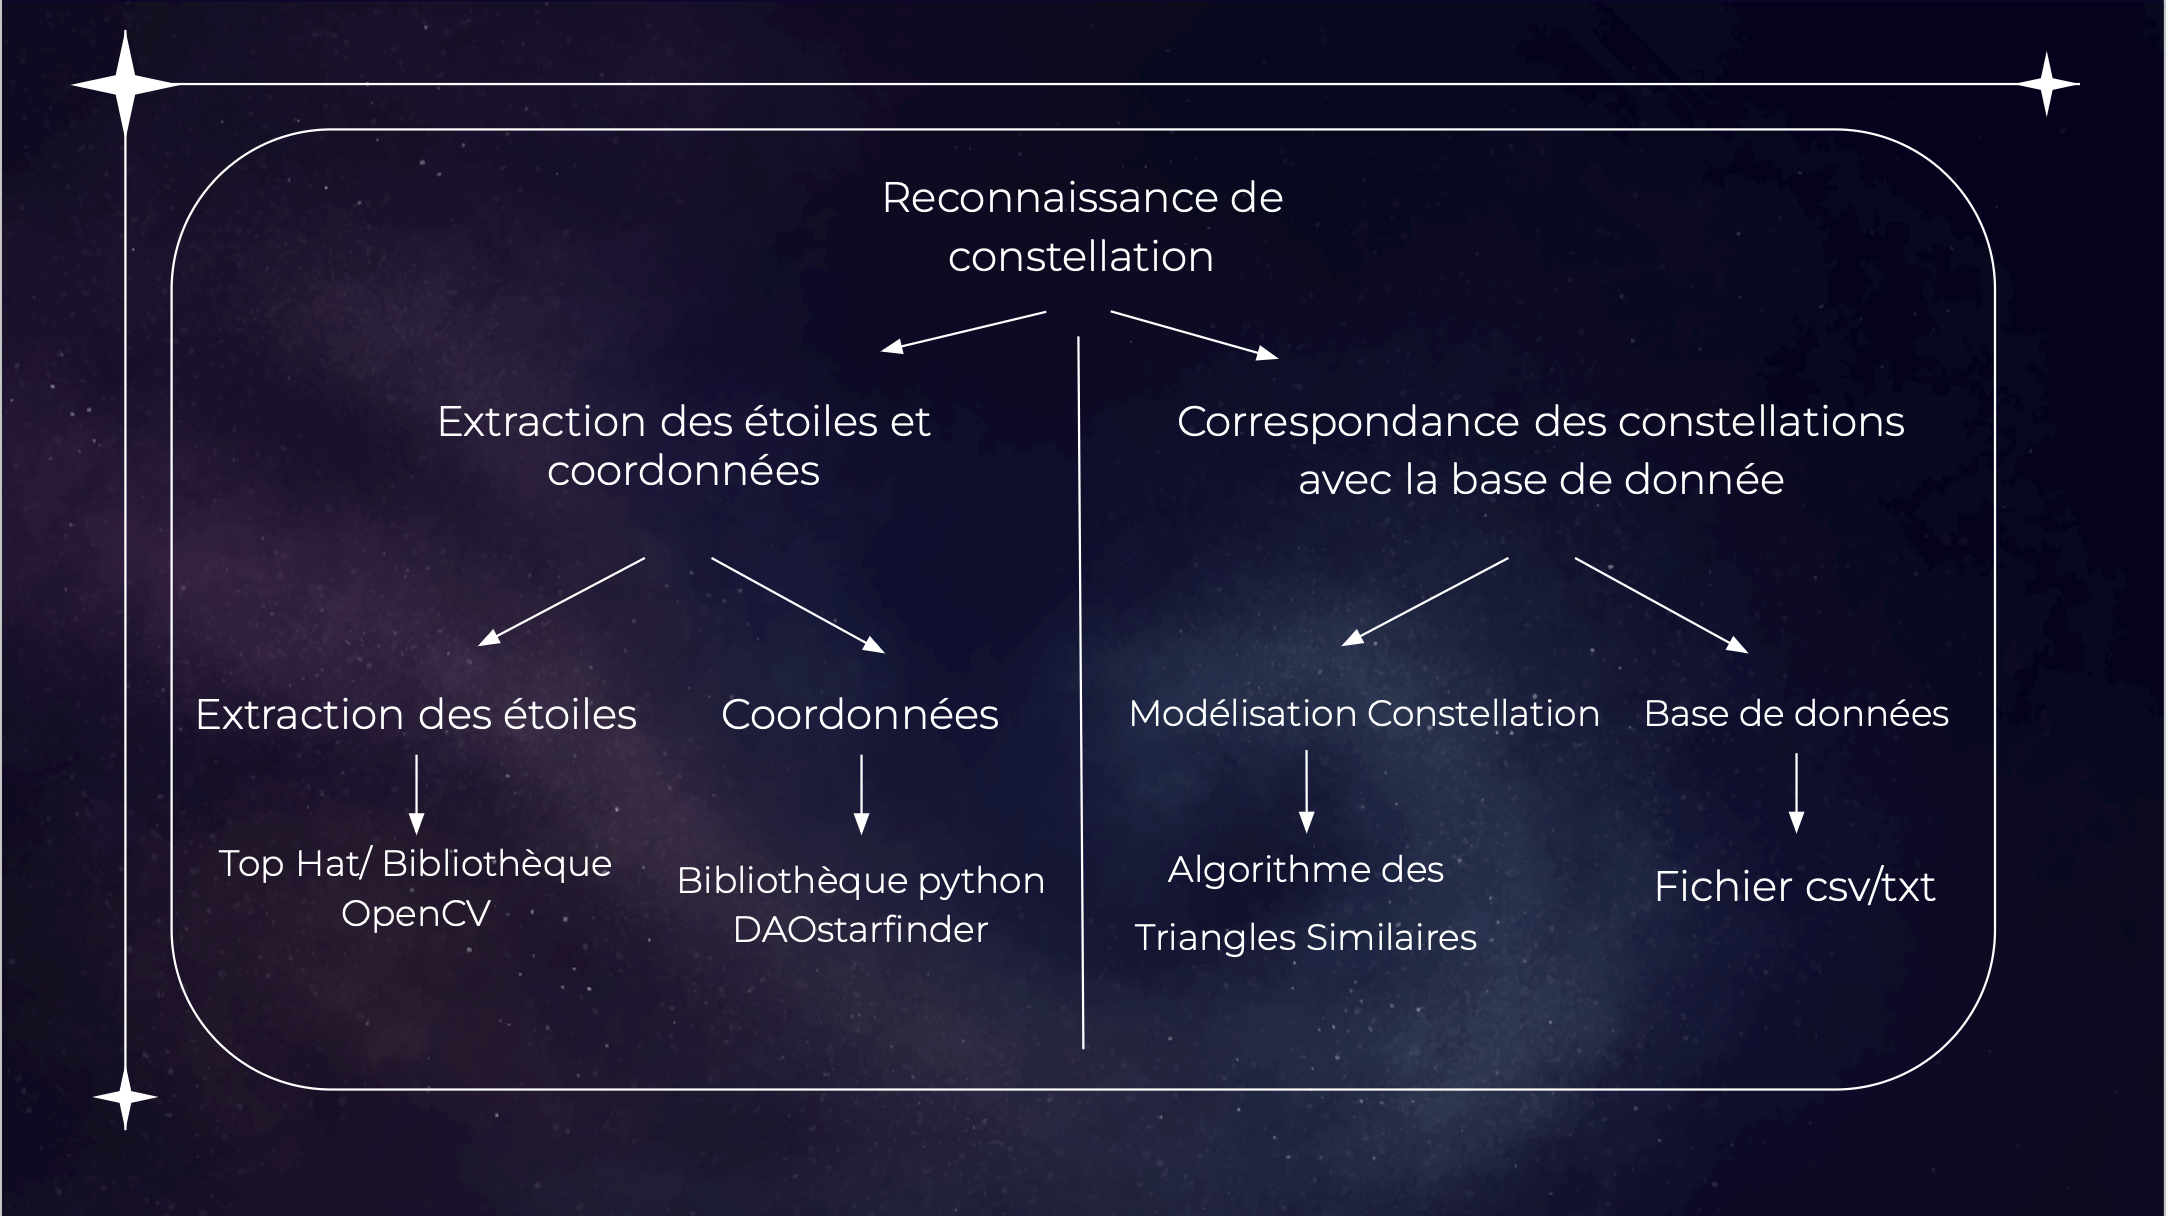
\includegraphics[width = 0.8\linewidth]
    {img/orga.png}
    \caption{Schéma d'organisation de la partie reconnaissance.}
\end{figure}

La partie algorithmique de reconnaissance de constellation est partagée par \textbf{deux langages} qui exploitent chacun leur plus grande force. En effet, \textbf{l'extraction d'étoiles et la manipulation d'image sont gérés par Python} et ses librairies tandis que \textbf{le corps du programme est en Java}. On profite de l'optimisation de Python pour les calculs et la structure de classes de Java. En réalité, suite à la création de l'interface, le projet est passé à une structure Maven et l'interface est devenue le centre de commande du logiciel.
 
\subsubsection{Interface}

 D'abord en JavaSwing, l'interface a évolué en JavaFx pour des raisons de praticité et surtout car JavaSwing n'est plus mis à jour.
 
\begin{figure}[ht]
    \centering
    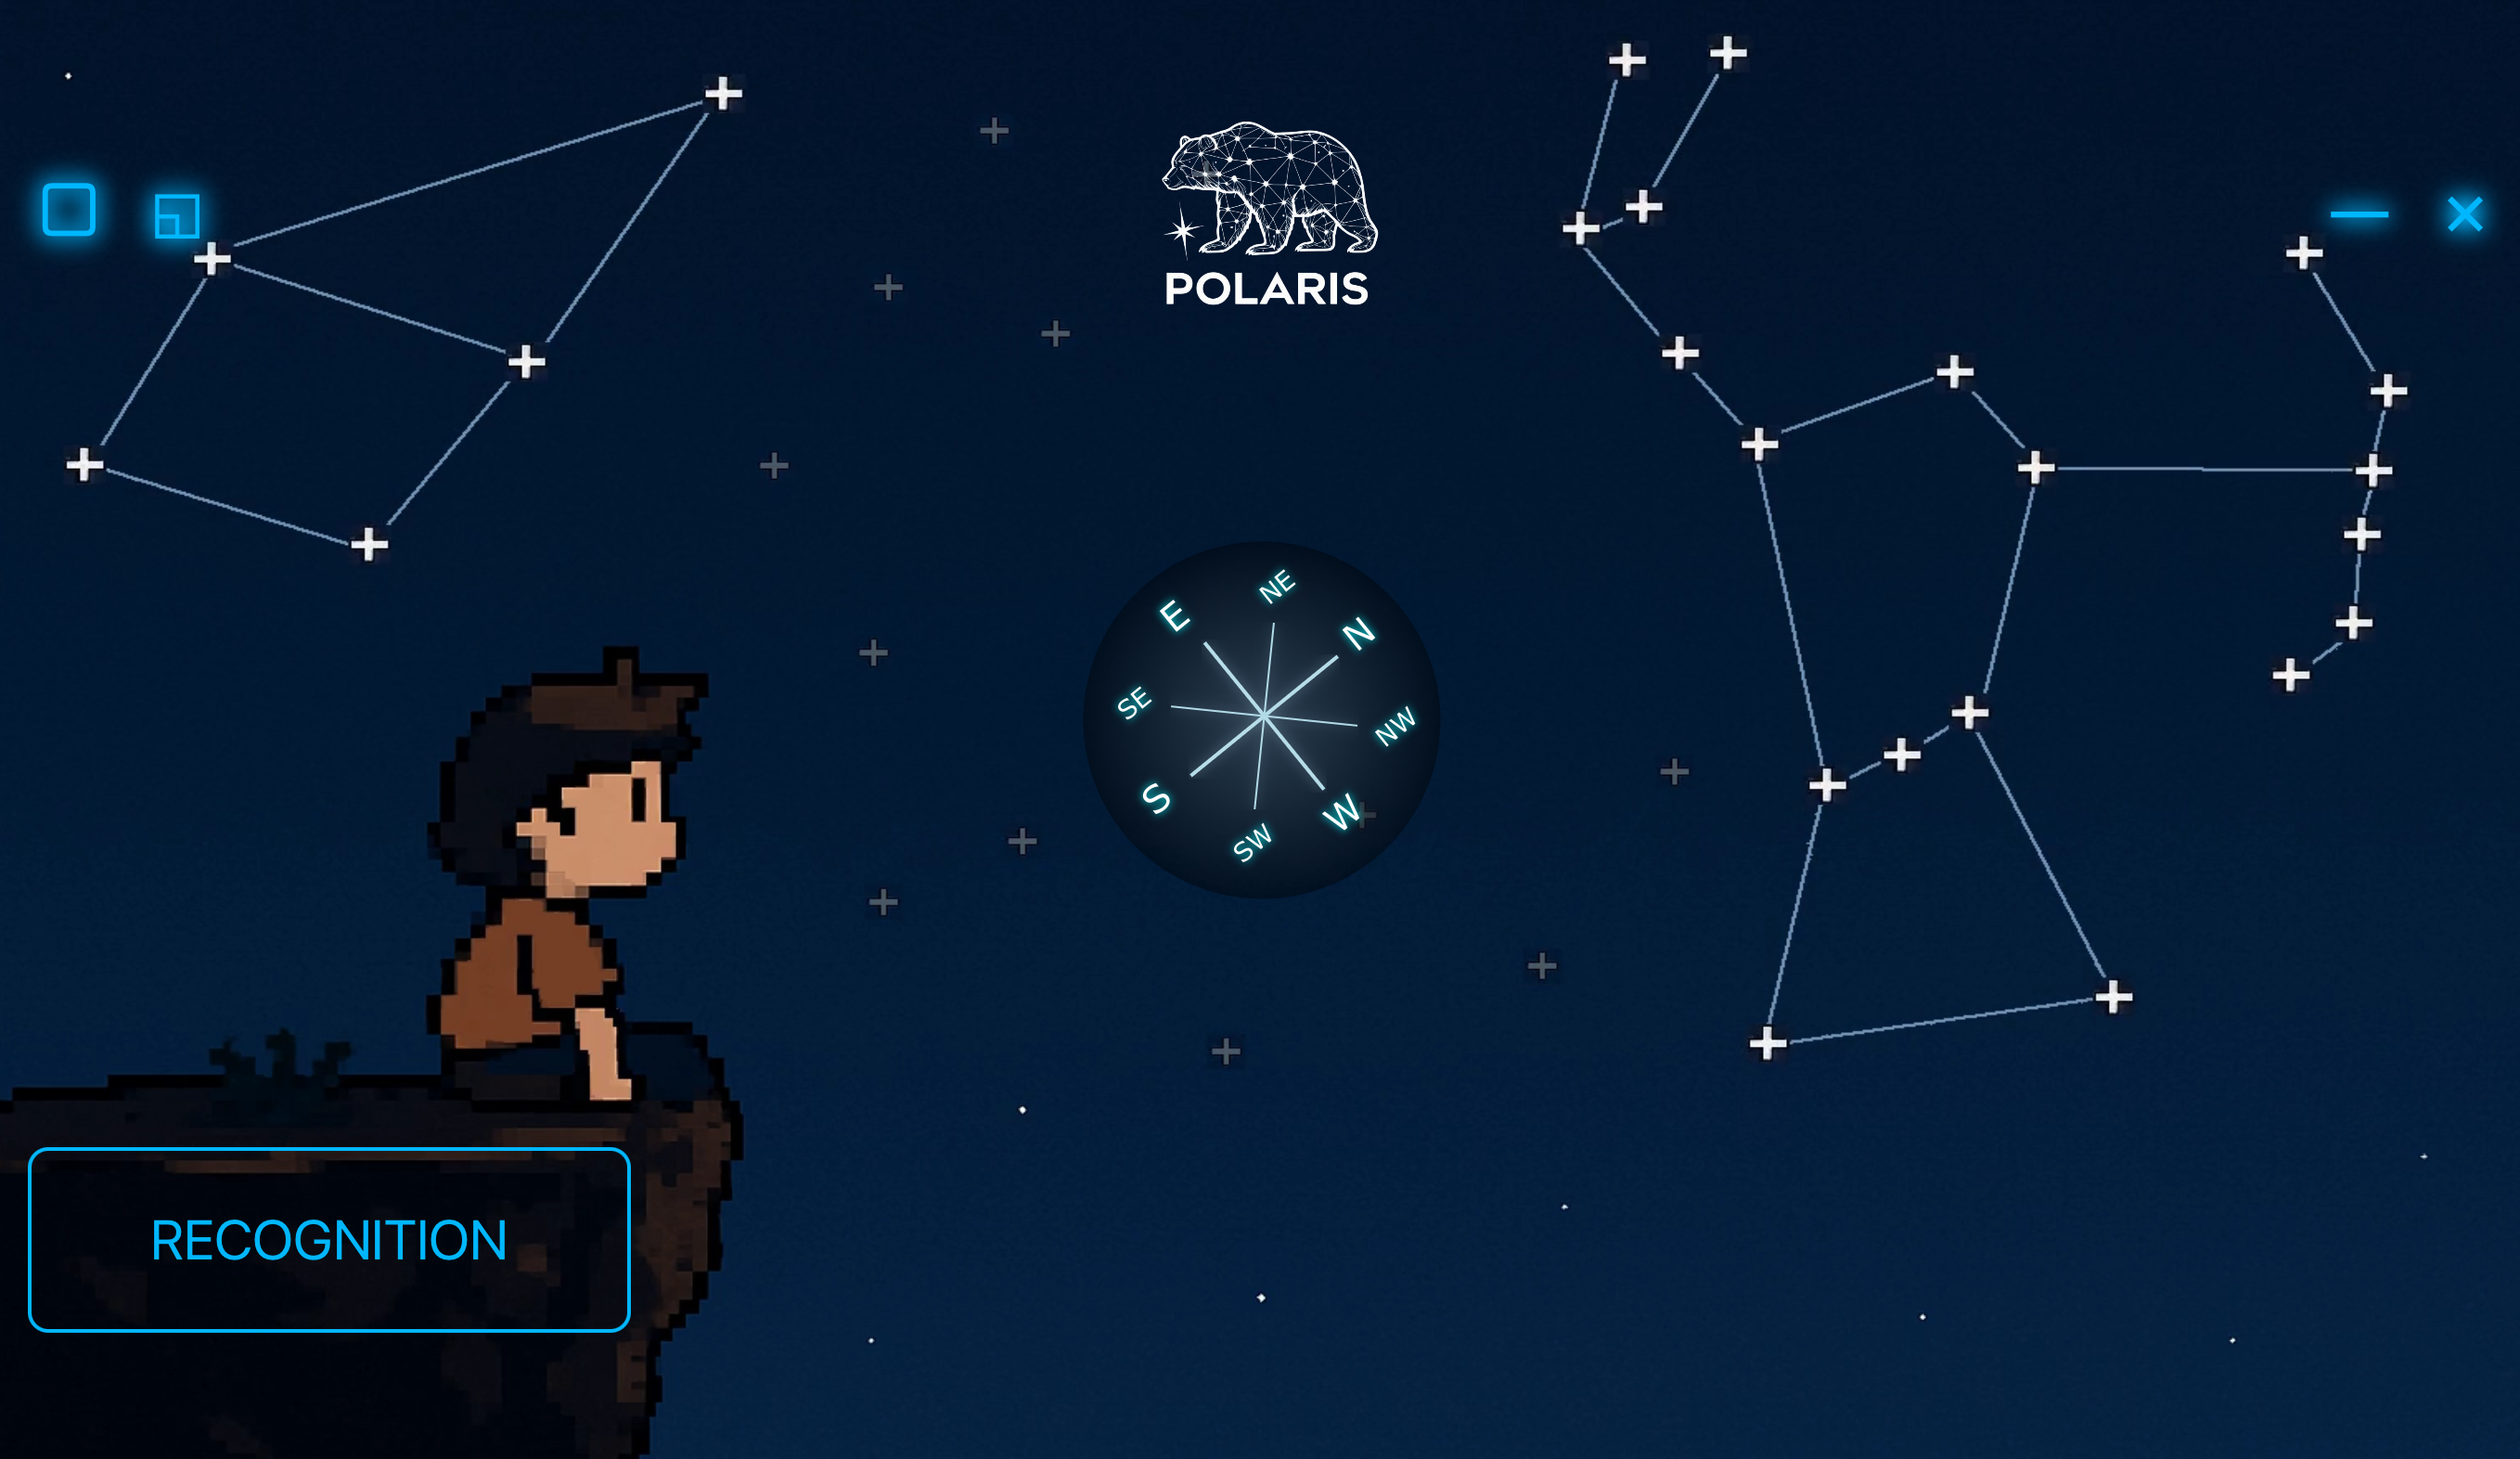
\includegraphics[width = 0.6\linewidth]{img/Interfacefinale.png}
    \caption{Interface du logiciel \textbf{\textit{Polaris}}}
\end{figure}

\subsubsection{Diagramme de classes}

Le diagramme de classe du projet contient les classes de la partie reconnaissance et de la partie interface. La partie Python ne contient pas de classes.

\begin{figure}[ht]
    \centering
    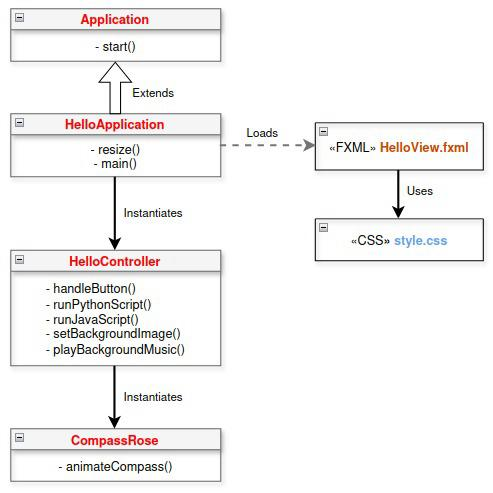
\includegraphics[width = 0.6\linewidth]{img/diagrammeclasseinterface.jpeg}
    \caption{Diagramme de l'interface (Apparaissent seulement les méthodes essentielles)}

    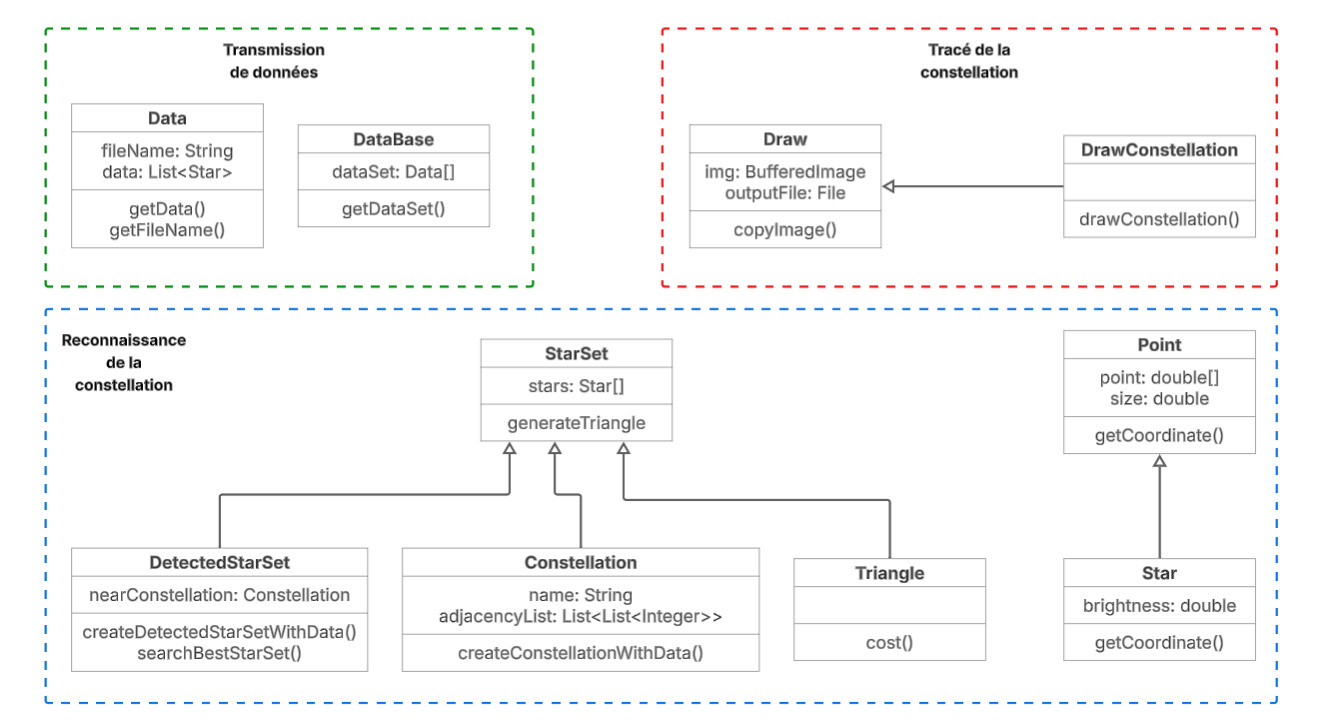
\includegraphics[width = 0.8\linewidth]{img/diagrammeclasserecognition.jpeg}
    \caption{Diagramme de la partie reconnaissance (Apparaissent seulement les méthodes essentielles)}
\end{figure}

\subsection{Choix des Technologies}

\textbf{Logiciel de version}

\vspace{0.2cm}

\noindent \textbf{GitHub} pour la collaboration et la gestion du code source.

\vspace{0.3cm}

\textbf{Langages de Programmation}

\vspace{0.2cm}

\noindent \textbf{Python} pour la détection d'étoile (traitement d'image). 

\textbf{ Bibliothèques} : DAOStarFindfer (Pillow), NumPy qui est une bibliothèque adaptée à notre problématique.

\vspace{0.2cm}

\noindent \textbf{Java} pour la reconnaissance de constellation et interface : rapide et performant.

\textbf{ Bibliothèques} : JavaFx pour la praticité du fxml, les compatibilités CSS, etc.

\vspace{0.3cm}

\textbf{Tests Unitaires}

\vspace{0.2cm}

\noindent \textbf{JUnit} : framework gratuit et open source pour les tests unitaires Java

\vspace{0.2cm}

\noindent \textbf{Unittest} : framework pour les tests unitaires Python

\vspace{0.3cm}

\textbf{IDE}

\vspace{0.2cm}

\noindent \textbf{VScode} pour plus de flexibilité pour passer d'un langage à un autre  

\vspace{0.3cm}

\textbf{Autres outils utilisés finalement abandonnés pour de meilleurs}

\vspace{0.2cm}

\noindent \textbf{Bibliothèques} : JavaSwing pour apprendre les bases de l'interface via Java

\vspace{0.2cm}

\noindent \textbf{Format de transmission de données} : Json pour l'échange de données en texte lisible

\vspace{0.2cm}

\noindent \textbf{IDE : Apache Netbeans} pour l'interface Java Swing.

\subsection{Gestion de projet}
\textbf{Diagramme de Gantt}

Le projet Polaris a rapidement trouvé ses 4 membres et l'équipe a donc pu commencer le brainstorming et la bibliographie dès fin septembre. Le plan de charge du projet pourra être retrouvé en annexe. 

\begin{figure}[ht]
    \centering    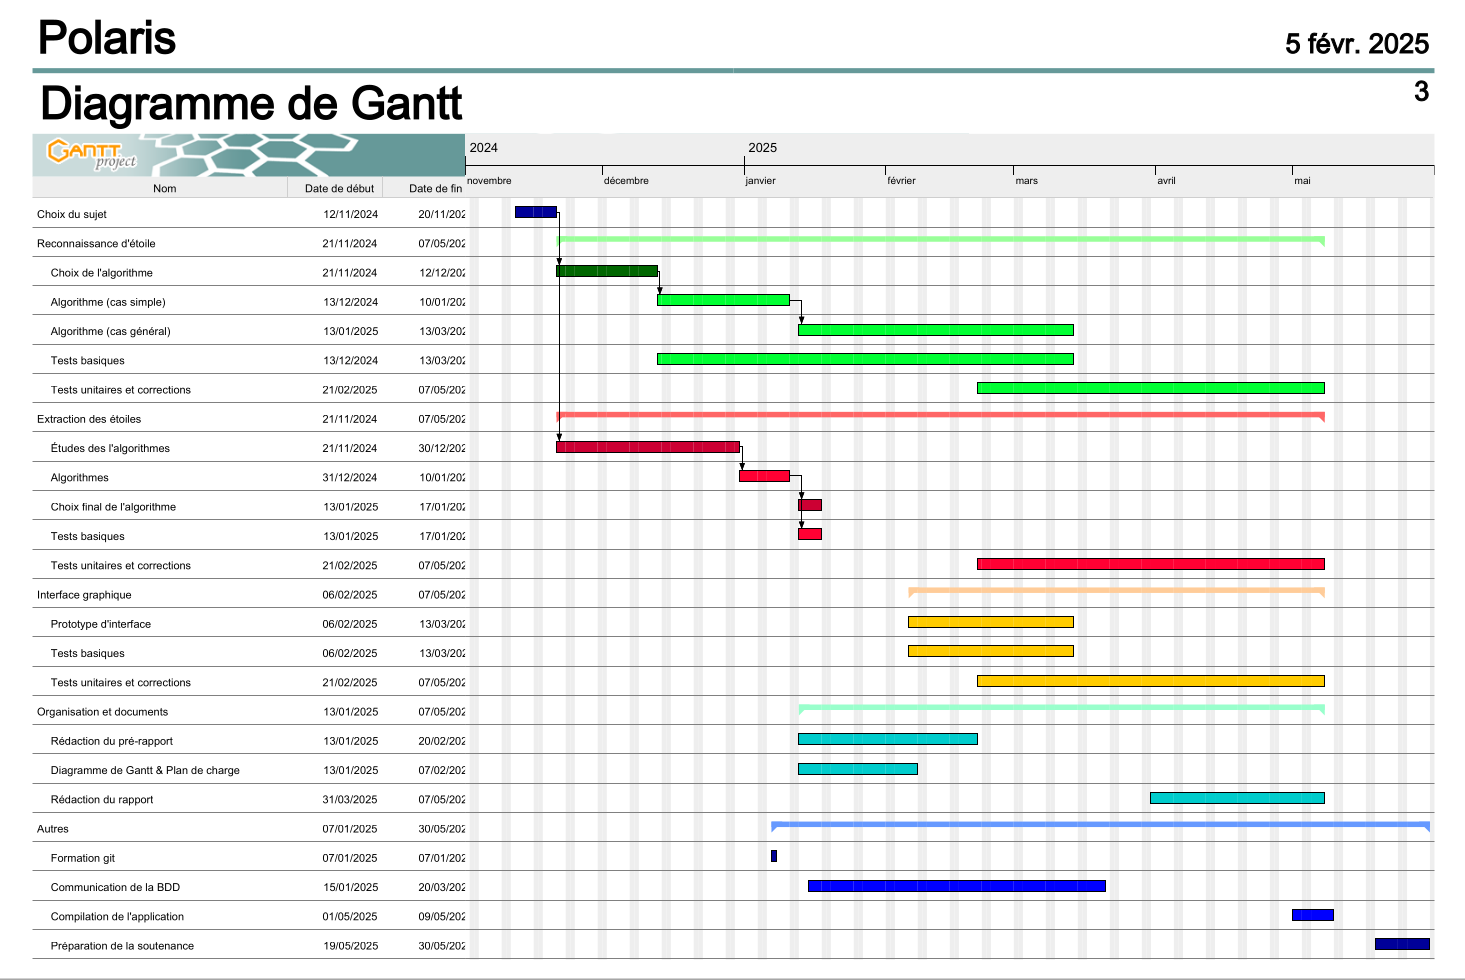
\includegraphics[width=0.8\linewidth] {img/Gantt2.png}  
    \caption{Diagramme de Gantt}  
\end{figure}